
%\begin{center}
    \section{\Large{Лекция 1}}
    \subsection{\large{ Введение. Основные понятия}}
%\end{center}
\begin{Def}
\fcolorbox{g}{g}{Дифференциальное уравнение (ДУ)} --- уравнение, связывающее \begin{itemize}
    \item значения производных функций, порядок которых формально ничем не ограничен
    \item с самими функциями
    \item со значениями независимых переменных.
\end{itemize}
\end{Def}

\vspace{3mm}

\begin{example}
ДУ 2-го порядка:
$y'' + (y')^2 + \cfrac{1}{y} = x^2 - 1$
\end{example}

\fcolorbox{p}{p}{!} $y' = \cfrac{dy}{dx}$ не является ДУ! Это дифференциальное тождество.

\vspace{5mm}
\begin{Def}
\fcolorbox{g}{g}{Порядком ДУ} называют наивысший порядок производной, входящей в это уравнение.
\end{Def}

\vspace{3mm}

\begin{example}
$(y')^3 + \cfrac{1}{y} = x$ --- ДУ 1-го порядка.
\end{example}

\begin{example}
Волновое уравнение: $U_t = a^2 U_{xx}$
\end{example}

В предыдущих примерах независимой переменной была $x$, здесь же их две: $x, t$.

\vspace{5mm}

\begin{Def}
ДУ, выражающее зависимость между
\begin{itemize}
    \item независимой переменной (одной!) (аргумент),
    \item зависимой переменной (функция),
    \item одной или более производными функций
\end{itemize}
называют \fcolorbox{g}{g}{обыкновенным дифференциальным уравнением (ОДУ)}.
\end{Def}
\newpage
\begin{Def}
ДУ, содержащее в себе
\begin{itemize}
    \item завсимую переменную,
    \item две или более независимых переменных
    \item вместе с частными производными зависимой переменной относительно независимых
\end{itemize}
называется \fcolorbox{g}{g}{ДУ в частных производных (ДУЧП)}.
\end{Def}
\begin{center}
    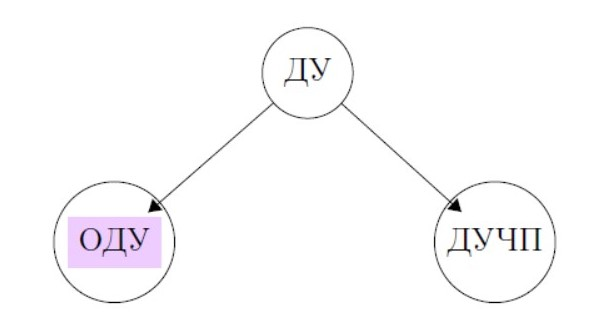
\includegraphics[width=0.4\textwidth]{p1.jpg}
\end{center}

\textbf{Обозначения:}
\begin{itemize}
    \item $x$ --- независимое переменное
    \item $y = y(x)$ --- зависимое переменное (функция)
    \item $y'(x) = \cfrac{dy}{dx}$, $y''(x) = \cfrac{d^2y}{dx^2}$ и т. д.
    \item $\vec{y} = \vec{y}(x) = 
    \begin{pmatrix}
    y_1(x)\\
    y_2(x)\\
    \ldots\\
    y_n(x)
    \end{pmatrix}$, 
    $\vec{y'} = \cfrac{\vec{dy}}{dx} = 
    \begin{pmatrix}
    dy_1/dx\\
    dy_2/dx\\
    \ldots\\
    dy_n/dx
    \end{pmatrix} = 
    \begin{pmatrix}
    y_1'\\
    y_2'\\
    \ldots\\
    y'_n
    \end{pmatrix}$ --- если искомых функций несколько.
\end{itemize}

\vspace{5mm}

\begin{Def}
Уравнение вида
\begin{equation}\label{1.1}
    F(x, y(x, y'(x), \ldots, y^{(n)}(x)) = 0,
\end{equation} связывающее
\begin{itemize}
    \item независимое переменное $X$,
    \item искомую функцию $y = y(x)$,
    \item её производные $y'(x), \ldots, y^{(n)}(x)$
\end{itemize}
называется \fcolorbox{g}{g}{обыкновенным ДУ в общем виде}.
\end{Def}
\vspace{3mm}

\textbf{Ещё обозначения:}
\begin{itemize}
    \item $x \in I$, где $I$ --- $(a,b)$, $[a,b)$, $(a, b]$ (интервалы могут быть конечные и бесконечные) или $[a,b]$
    \item $C(I)$ --- множество непрерывных на $I$ функций
    \item $C^k(I)$ --- множество $k$ раз непрерывно дифференцируемых на $I$ функций


\item Рассмотрим
$D \subset \R^n_{\vec{y}}$, $D:$ $ I \xrightarrow{\vec{y}(x)} \R^n_{\vec{y}}$

$G = I \times D \subset \R^{1 + n}_{x, \vec{y}}$

$\Omega \subset \R^{n + 2}_{x, y, y', \ldots, y^{(n)}}$, $\Tilde{\Omega} \subset \R^{n + 1}_{x, y, y', \ldots, y^{(n - 1)}}$
\end{itemize}

\textbf{Если не оговорено противное, в дальнейшем полагаем:}
$F(x, y, y', \ldots,y^{(n)}) \in C(\Omega)$.

\vspace{5mm}

\textbf{\underline{Наша цель:}} найти решение уравнения \ref{1.1}.

\begin{Def}
\fcolorbox{g}{g}{Решением ОДУ (\ref{1.1})} на $I$ называется функция $y = \varphi (x)$, заданная на $I$, если:
\begin{enumerate}
    \item $\varphi (x) \in C^n (I)$
    \item $\forall x \in I$ точка $(x, y(x), y'(x), \ldots,y^{(n)}(x) ) \in \Omega$
    \item $F(x, \varphi(x), \varphi'(x), \ldots, \varphi^{(n)}(x)) \equiv 0$ $\forall x \in I$
\end{enumerate}
\end{Def}

\vspace{3mm}

\begin{Def}
График у= решения ОДУ \ref{1.1} $y = \varphi(x)$, $x \in I$ на плоскости $\R^2_{x, y}$ называется \fcolorbox{g}{g}{интегральной кривой ОДУ \ref{1.1}}.
\end{Def}

Решение не всегда представляется в виде интегральной кривой.

\begin{example}
(из домашки) $(x - 1)y' + y(y + 1) = 0$

Решение: $\cfrac{y}{y + 1} = C(x + 1)$ и $y = 1$.

Здесь $y$ не выражается в явном виде как функция $x$. В таких случаях говорят: имеем решение в виде интеграла:

$\Phi(x, y, C) = 0$ определяет $y$ как неявную функцию от $x$.
\end{example}

\begin{note}
Если уравнение $n$-го порядка, то обычно интеграл содержит $n$ произвольных постоянных:

$\Phi(x, y, C_1, \ldots, C_n) = 0$.
\end{note}

Итак, \textbf{интегральная кривая --- всегда  интеграл, но интеграл может не быть интегральной кривой.}

\vspace{5mm}

Уравнение \ref{1.1} $F(x, y, y', \ldots, y^{(n)} ) = 0$ можно разрешить относительно $y^{(n)}$.
\begin{equation}\label{1.2}
    y^{(n)} = f(x, y, y', \ldots, y^{(n - 1)})
\end{equation}

\begin{Def}
ОДУ \ref{1.2}, разрешенное относительно \textbf{старшей} производной, называется \fcolorbox{g}{g}{ОДУ в нормальной форме (виде) или ОДУ в форме (виде) Коши}.
\end{Def}

\vspace{3mm}

\textbf{Если не оговорено противное, то $f(x, y, y', \ldots, y^{(n - 1)}) \subset C(\Tilde{\Omega})$}.

\textbf{Наша задача --- отыскание всех решений и изучение их свойств.}

\begin{example}\label{ex5}
$(y')^2 - 2xy' = x^2 - 4y$

Решение: $y = \cfrac{x^2}{2}$, $y = \cfrac{1}{4}(C^2 - 2(x - c)^2)$
\end{example}
\vspace{3mm}
\begin{example}\label{ex6}
$(e^x + 1)^2y' + (e^{2x} - 1)y)$

Решение: $y = C \cfrac{e^x}{(1 + e^x)^2}$
\end{example}

Важно не терять решения, которые не задаются общей формулой.

\textbf{В чём отличие \ref{ex5} и \ref{ex6}?}

Решение в \ref{ex6} --- параметрическое семейство интегральных кривых. Для любого решения этого ДУ найдется такое значение $C$, что интегральная кривая совпадает с решением.
 
Решение в \ref{ex6} --- 1-параметрическое семейство кривых: $C$ эксклюзивная постоянная.

Подробнее об этом будет попозже.

\vspace{3mm}

\begin{Def}
\fcolorbox{g}{g}{Общее решение ОДУ \ref{1.1}, \ref{1.2}} --- решение, зависящее от $n$ произвольных постоянных $c_1, \ldots, c_n$: $y = \varphi(x, c_1, \ldots, c_n)$. При этом
\begin{itemize}
    \item Любому набору $c_1, \ldots, c_n$ соответствует решение.
    \item Для любого решения существует соответствующий набор $c_1*, \ldots, c_n*$.
\end{itemize}
\end{Def}

\ref{ex6} получено общее решение. А решение \ref{ex5} общим не является. Оно называется \textbf{однопараметрическим семейством решений}.

\begin{Def}
Каждое решение ОДУ \ref{1.1}, \ref{1.2}, которое получается из общего (или из $n$-параметрического семейства решений) $y = \varphi(x, c_1, \ldots, c_n)$ при придавании постоянным $c_1, \ldots, c_n$ определенных значений, будем называть \fcolorbox{g}{g}{частным решением}.
\end{Def}

\vspace{3mm}

\ref{ex5}: Пусть $C = 0$. $y = \cfrac{-x^2}{2}$ --- частное решение.

\ref{ex6}: Пусть $C = 0$. $y = 0$ --- тоже частное решение.

\vspace{3mm}

По аналогии вводятся понятия \textbf{общего интеграла} (для ДУ, где $y$ выражается неявно) и \textbf{$n$-параметрическое семейство интегралов}.

\vspace{5mm}

\subsection{\large{ОДУ 1-го порядка}}   

\begin{itemize}
    \item основные понятия
    \item ОДУ 1-го порядка, интегрируемые в конечном виде
\end{itemize}

ОДУ 1-го порядка в \fcolorbox{g}{g}{общем виде}:
\begin{equation}\label{2.1}
    F(x, y(x), y'(x)) = 0
\end{equation}

ОДУ 1-го порядка \fcolorbox{g}{g}{в виде Коши (в нормальной форме)}:
\begin{equation}\label{2.2}
    y'(x) = f(x, y)
\end{equation}

\vspace{3mm}

\textbf{Обозначения:}
\begin{itemize}
    \item $x \in I$, где $I$ --- $(a,b)$, $[a,b)$, $(a, b]$,$[a,b]$
    \item $D:$ $ I \xrightarrow{\vec{y}(x)} \R^n_{\vec{y}}$
    \item $G = I \times D$, $(x, y) \in G$
    \item $(x, y, y') \in \Omega \in \R^3$, $\Tilde{\Omega} = G$
\end{itemize}
\newpage
\begin{center}
\textbf{\large{1. Простейший  случай}}
\end{center}
\begin{equation}\label{2.3}
    y' = f(x)
\end{equation}
Все решения: $ \displaystyle t (x) = \int\limits_{x_0}^x f(\xi)d\xi + C$; $x, x_0 \in I$

\vspace{3mm}

\textbf{Процесс нахождения решений ДУ называется интегрированием ДУ.}

\begin{Def}
    ДУ, интегрируемые при помощи конечного числа интегралов или других элементарных действий (операций), называются \fcolorbox{g}{g}{интегрируемыми в квадратурах} или в конечном виде.
\end{Def}

\ref{2.3} является интегрируемым в квадратурах.

\begin{example}
    Семейство $y = \tg(x + c)$ --- решение уравнения $y' = y^2 + 1$.
    
    Знаем: $\brackets{x + c} \in \brackets{-\cfrac{\pi}{2} + \pi k; \cfrac{\pi}{2} + \pi k}$
    
    Значит, $x \in \brackets{-\cfrac{\pi}{2} + \pi k - c; \cfrac{\pi}{2} + \pi k - c}$
    
    Придавая постоянной $c$ разные значения, будем получать разные промежутки.
\end{example}
\vspace{4mm}

\begin{center}
\textbf{\large{2. Уравнение с разделяющимися переменными}}
\end{center}
\begin{equation}\label{2.4}
    y' = f(y)
\end{equation}

Если $f(y) \neq 0$: $\cfrac{dy}{f(y)} = dx$ --- уравнение с разделенными переменными.

$\displaystyle \int\cfrac{dy}{f(y)} + c = x$

\textbf{??? Почему можно интегрировать???}

Если $f(y*) = 0$, $y* = const$

$\cfrac{dy*}{dx} = 0 = f(y*) \Rightarrow y* = const$ --- тоже решение.

\begin{example}
    $y' = y^2 + 1$
    
    Повезло: $f(y) = y^2 + 1 \neq 0$
    
    $\cfrac{dy}{y^2 + 1} = dx$
    
    $\arctg y = x + c$
    
    $y = \tg (x + c)$
    
    В обратную сторону: какому ДУ соответствует решение $y = tg(x + c)$? Избавимся от $c$.
    
    Дифференцируем: $y' = \cfrac{1}{\cos^2(x + c)}$. Помним: $\tg^2(x + c) + 1 = \cfrac{1}{\cos^2(x + c)}$
    
    Отсюда: $y' = y^2 + 1$.
\end{example}
\vspace{3mm}

\textbf{Бывают грустные ситуации \Frowny}

$y' + y^2 = x^2$ --- уравнение Риккати (специальное).

Лиувилль доказал: $y' + y^2 = x^a$ интегрируемо в квадратуре тогда и только тогда, когда $a = \cfrac{-4n}{2n - 1}$, $n \in \Z$ или $a = -2$.

Что делать в остальных случаях?

\Smiley Численные методы узнаем на 3 курсе. А сейчас будем использовать \textbf{метод изоклин}. Он не дает точного решения, но позволяет сделать прогнозы относительно поведения функций.

\begin{center}
    \textbf{Геометрический смысл $y' = f(x, y)$}
\end{center}
\begin{figure}[!ht]
		\centering
		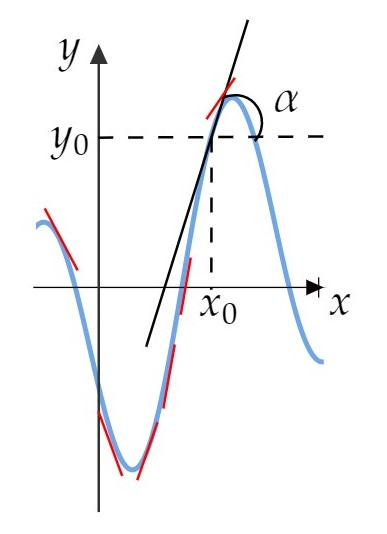
\includegraphics[width=0.3\textwidth]{images/p2.jpg}
\end{figure}

$\tg \alpha = y' |_{(x_0, y_0)}$ --- каждой точке соответствует отрезочек касательной.

$\cfrac{1}{f(x_i, y_i)}$ --- отрезок коллинеарен.

Множество всех отрезков --- \textbf{поле направлений}.
\begin{problem}
    Дано семейство кривых: $y = c \cos x + 2$. Найти ортогональные траектории.
    
    $y' = f(x,y)$
    
    Поле направлений: $\brackets{\cfrac{1}{f(x_i, y_i)}} = \vec{a}$ (а)
    
    Ортогональные траектории: $y' = g(x, y)$ (б), поле направлений: $\brackets{\cfrac{1}{g(x_i, y_i)} }= \vec{b}$
    \begin{figure}[!ht]
		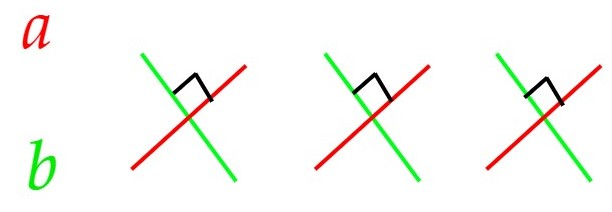
\includegraphics[width=0.2\textwidth]{images/p3.jpg}
\end{figure}
$\vec{a} \perp \vec{b}$, $(\vec{a}, \vec{b}) = 0 = 1 + fg \Rightarrow g = -\cfrac{1}{f}$

Осталось проинтегрировать б.

а: $y = c \cos x + 2$

$y' = -c \sin x$

$c = -\cfrac{y'}{\sin x} = \cfrac{y - 2}{\cos x} \Rightarrow y' = (2 - y) \tg x$

$f = (2 - y) \tg x$

$g = \cfrac{\ctg x}{y - 2}$, $y' = \cfrac{\ctg x}{y - 2}$
\end{problem}

\begin{center}
\textbf{\large{2. Следующий случай}}
\end{center}

\begin{equation}
    y' = f(x, y) = f_1(x)f_2(y)
\end{equation}

$dx \neq 0$. Если $f_1(x*) = 0$: $x* = const*$ --- не решение по ОДЗ.

Если $f(y*) = 0$, $y* = const*$ --- решение.

$\cfrac{dy}{f_2(y)} = f_1(x) dx$

$ \displaystyle \int\cfrac{dy}{f_2(y)} = \int f_1(x) dx + c$ --- решение в виде интеграла.

??? Почему можно интегрировать ??? --- аналогично предыдущему случаю.

\begin{example}
    $(y - 2)dy = \cfrac{cosx\ dx}{sinx}$
    
    $\displaystyle \cfrac{y^2}{2} - 2y = \int\cfrac{dsinx}{sinx} = \ln|sinx| + c$, $c \in \R$ --- семейство ортогональных траекторий в виде и нтеграла.
\end{example}